% This file was created by matplotlib2tikz v0.6.18.
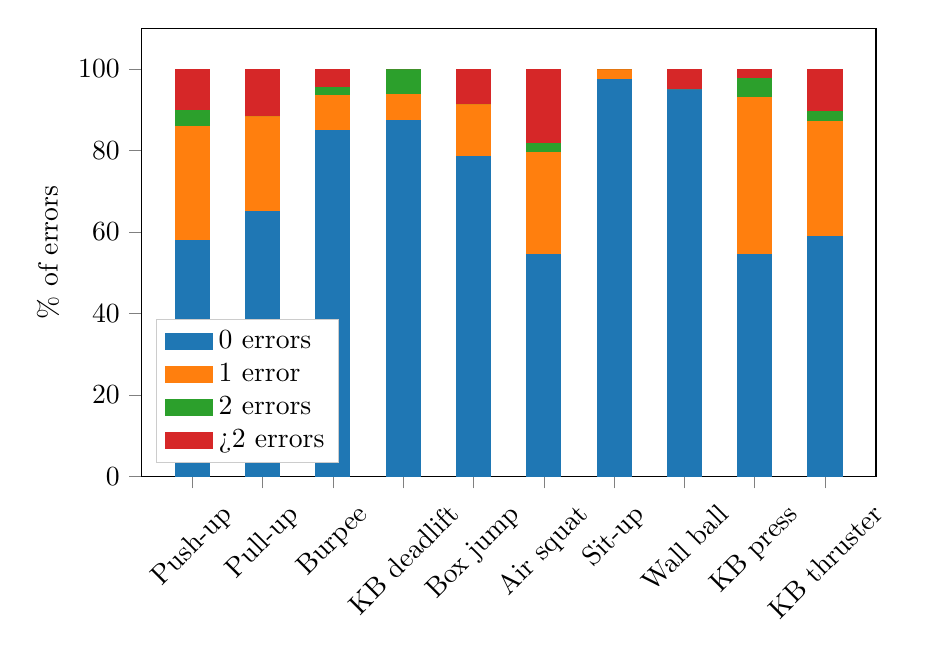
\begin{tikzpicture}

\definecolor{color1}{rgb}{1,0.498039215686275,0.0549019607843137}
\definecolor{color0}{rgb}{0.12156862745098,0.466666666666667,0.705882352941177}
\definecolor{color3}{rgb}{0.83921568627451,0.152941176470588,0.156862745098039}
\definecolor{color2}{rgb}{0.172549019607843,0.627450980392157,0.172549019607843}

\begin{axis}[
width=0.9\textwidth,
height=0.6\textwidth,
legend cell align={left},
legend style={at={(0.02,0.03)}, anchor=south west, draw=white!80.0!black, fill opacity=1, draw opacity=1,text opacity=1},
tick align=outside,
tick pos=left,
xticklabel style={rotate=45},
x grid style={lightgray!92.026143790849673!black},
xmin=-0.725, xmax=9.725,
xtick={0,1,2,3,4,5,6,7,8,9},
xticklabels={Push-up,Pull-up,Burpee,KB deadlift,Box jump,Air squat,Sit-up,Wall ball,KB press,KB thruster},
y grid style={lightgray!92.026143790849673!black},
ylabel={\% of errors},
ymin=0, ymax=110
]
\addlegendimage{color0, fill=color0, area legend}
\addlegendentry{0 errors}
\addlegendimage{color1, fill=color1, area legend}
\addlegendentry{1 error}
\addlegendimage{color2, fill=color2, area legend}
\addlegendentry{2 errors}
\addlegendimage{color3, fill=color3, area legend}
\addlegendentry{>2 errors}
\draw[fill=color0,draw opacity=0] (axis cs:-0.25,0) rectangle (axis cs:0.25,58);
\draw[fill=color0,draw opacity=0] (axis cs:0.75,0) rectangle (axis cs:1.25,65.1);
\draw[fill=color0,draw opacity=0] (axis cs:1.75,0) rectangle (axis cs:2.25,85.1);
\draw[fill=color0,draw opacity=0] (axis cs:2.75,0) rectangle (axis cs:3.25,87.5);
\draw[fill=color0,draw opacity=0] (axis cs:3.75,0) rectangle (axis cs:4.25,78.72);
\draw[fill=color0,draw opacity=0] (axis cs:4.75,0) rectangle (axis cs:5.25,54.54);
\draw[fill=color0,draw opacity=0] (axis cs:5.75,0) rectangle (axis cs:6.25,97.62);
\draw[fill=color0,draw opacity=0] (axis cs:6.75,0) rectangle (axis cs:7.25,95.2);
\draw[fill=color0,draw opacity=0] (axis cs:7.75,0) rectangle (axis cs:8.25,54.54);
\draw[fill=color0,draw opacity=0] (axis cs:8.75,0) rectangle (axis cs:9.25,58.97);
\draw[fill=color1,draw opacity=0] (axis cs:-0.25,58) rectangle (axis cs:0.25,86);
\draw[fill=color1,draw opacity=0] (axis cs:0.75,65.1) rectangle (axis cs:1.25,88.4);
\draw[fill=color1,draw opacity=0] (axis cs:1.75,85.1) rectangle (axis cs:2.25,93.6);
\draw[fill=color1,draw opacity=0] (axis cs:2.75,87.5) rectangle (axis cs:3.25,93.75);
\draw[fill=color1,draw opacity=0] (axis cs:3.75,78.72) rectangle (axis cs:4.25,91.49);
\draw[fill=color1,draw opacity=0] (axis cs:4.75,54.54) rectangle (axis cs:5.25,79.54);
\draw[fill=color1,draw opacity=0] (axis cs:5.75,97.62) rectangle (axis cs:6.25,100);
\draw[fill=color1,draw opacity=0] (axis cs:6.75,95.2) rectangle (axis cs:7.25,95.2);
\draw[fill=color1,draw opacity=0] (axis cs:7.75,54.54) rectangle (axis cs:8.25,93.18);
\draw[fill=color1,draw opacity=0] (axis cs:8.75,58.97) rectangle (axis cs:9.25,87.18);
\draw[fill=color2,draw opacity=0] (axis cs:-0.25,86) rectangle (axis cs:0.25,90);
\draw[fill=color2,draw opacity=0] (axis cs:0.75,88.4) rectangle (axis cs:1.25,88.4);
\draw[fill=color2,draw opacity=0] (axis cs:1.75,93.6) rectangle (axis cs:2.25,95.7);
\draw[fill=color2,draw opacity=0] (axis cs:2.75,93.75) rectangle (axis cs:3.25,100);
\draw[fill=color2,draw opacity=0] (axis cs:3.75,91.49) rectangle (axis cs:4.25,91.49);
\draw[fill=color2,draw opacity=0] (axis cs:4.75,79.54) rectangle (axis cs:5.25,81.81);
\draw[fill=color2,draw opacity=0] (axis cs:5.75,100) rectangle (axis cs:6.25,100);
\draw[fill=color2,draw opacity=0] (axis cs:6.75,95.2) rectangle (axis cs:7.25,95.2);
\draw[fill=color2,draw opacity=0] (axis cs:7.75,93.18) rectangle (axis cs:8.25,97.72);
\draw[fill=color2,draw opacity=0] (axis cs:8.75,87.18) rectangle (axis cs:9.25,89.74);
\draw[fill=color3,draw opacity=0] (axis cs:-0.25,90) rectangle (axis cs:0.25,100);
\draw[fill=color3,draw opacity=0] (axis cs:0.75,88.4) rectangle (axis cs:1.25,100);
\draw[fill=color3,draw opacity=0] (axis cs:1.75,95.7) rectangle (axis cs:2.25,100);
\draw[fill=color3,draw opacity=0] (axis cs:2.75,100) rectangle (axis cs:3.25,100);
\draw[fill=color3,draw opacity=0] (axis cs:3.75,91.49) rectangle (axis cs:4.25,100);
\draw[fill=color3,draw opacity=0] (axis cs:4.75,81.81) rectangle (axis cs:5.25,99.99);
\draw[fill=color3,draw opacity=0] (axis cs:5.75,100) rectangle (axis cs:6.25,100);
\draw[fill=color3,draw opacity=0] (axis cs:6.75,95.2) rectangle (axis cs:7.25,100);
\draw[fill=color3,draw opacity=0] (axis cs:7.75,97.72) rectangle (axis cs:8.25,99.99);
\draw[fill=color3,draw opacity=0] (axis cs:8.75,89.74) rectangle (axis cs:9.25,100);
\end{axis}

\end{tikzpicture}